\documentclass{beamer}
\usetheme{Antibes}
\usepackage{xcolor, colortbl}
\usepackage{algorithm}
\usepackage[noend]{algpseudocode}
\usepackage{textcomp}
\usepackage{listings}
\usepackage{hyperref}
\usepackage{alltt}
\usepackage{tikz}
\usepackage{framed}
\usepackage{marvosym}
\usepackage{wasysym}
\usepackage{marvosym}
\usepackage{crayola}
\usepackage{mathpartir}
\usepackage{tabularx}
\usepackage[belowskip=-15pt,aboveskip=0pt]{caption}
\usepackage[skins]{tcolorbox}
\usepackage{multicol}
\usetikzlibrary{positioning,shapes,arrows, backgrounds, fit, shadows, automata}
\usetikzlibrary{decorations.markings}
%\usepackage{wasysym}
%\usepackage{marvosym}
\setbeamertemplate{footline}[frame number]
%\usecolortheme{fly}
\usefonttheme{serif}

\title[Sujit]{Lexical Analysis \\
Programming Languages}
\author{Sujit Kumar Chakrabarti}
\institute{IIITB}
\date{}


\definecolor{lightblue}{rgb}{0.8,0.93,1.0} % color values Red, Green, Blue
\definecolor{darkblue}{rgb}{0.4,0.3,1.0} % color values Red, Green, Blue
\definecolor{Blue}{rgb}{0,0,1.0} % color values Red, Green, Blue
\definecolor{darkgreen}{rgb}{0,0.7,0.2} % color values Red, Green, Blue
\definecolor{Red}{rgb}{1,0,0} % color values Red, Green, Blue
\definecolor{Pink}{rgb}{0.7,0,0.2}
\definecolor{links}{HTML}{2A1B81}
\definecolor{mydarkgreen}{HTML}{126215}
\newcommand{\highlight}[1]{{\color{Red}(#1)}}

\newcommand{\myheader}[1]{
	{\color{darkblue}
		\begin{Large}
			\begin{center}
				{#1}
			\end{center}
		\end{Large}
	}
}
\newcommand{\myminorheader}[1]{
	{\color{BrickRed}
		\begin{Large}
			{\fontfamily{\sfdefault}\selectfont\textbf{#1}}
		\end{Large}
	}
}

%\tikzstyle{input} = [coordinate]
%\tikzstyle{output} = [coordinate]


\tikzstyle{bb}=[%
      rectangle, draw=black, thick, fill=OliveGreen!30, drop shadow, align=center,
      text ragged, minimum height=2em, minimum width=2em, inner sep=6pt
]

\tikzstyle{inv}=[%
      rectangle, draw=none,  align=center,
      text ragged, minimum height=2em, minimum width=2em, inner sep=6pt
]

\tikzstyle{db}=[%
      ellipse, draw=black, thick, fill=pink, drop shadow, align=center,
      text ragged, minimum height=2em, inner sep=6pt
]

\tikzstyle{jn}=[%
      ellipse, draw=black, thick, fill=black
]

\tikzstyle{io}=[%
      trapezium, trapezium left angle=60, trapezium right angle=120, draw=black, thick, fill=brown, drop shadow,
      text ragged, minimum height=2em, minimum width=2em, inner sep=6pt, align=center
]

\tikzstyle{glio}=[%
      trapezium, trapezium left angle=60, trapezium right angle=120, draw=red, line width = 1mm, fill=brown, drop shadow,
      text ragged, minimum height=2em, minimum width=2em, inner sep=6pt
]
\tikzstyle{gl}=[%
      rectangle, draw=red, line width = 1mm, fill=lightblue, drop shadow,
      text ragged, minimum height=2em, minimum width=2em, inner sep=6pt
]

\tikzstyle{en}=[%
      rectangle, draw=black, thick, fill=none,
      text ragged, minimum height=2em, minimum width=2em, inner sep=6pt
]

\tikzstyle{sh}=[%
      rectangle, draw=gray, thick, fill=none, color = gray,
      text ragged, minimum height=2em, minimum width=2em, inner sep=6pt
]


\lstdefinestyle{javacode}{
	language = Java,
	basicstyle = \ttfamily\scriptsize,
	stringstyle = \ttfamily,
	keywordstyle=\color{Blue}\bfseries,
	identifierstyle=\color{Pink},
	commentstyle=\color{darkgreen},
	frame=single,
	frameround=tttt,
%	numbers=left
	showstringspaces=false
}

\lstdefinestyle{camlcode}{
	language = Caml,
	basicstyle = \scriptsize\ttfamily,
	stringstyle = \color{red}\ttfamily,
	keywordstyle=\color{Blue}\bfseries,
	identifierstyle=\ttfamily,
	frame=single,
	frameround=tttt,
	numbers=none,
	showstringspaces=false,
	escapeinside={(*@}{@*)}
}

\lstdefinestyle{outputcode}{
	language = bash,
	backgroundcolor = \color{black},
	basicstyle = \tiny\ttfamily\color{white},
	stringstyle = \color{red}\ttfamily,
	keywordstyle=\color{white}\bfseries,
	identifierstyle=\ttfamily,
	frameround=tttt,
	numbers=none,
	showstringspaces=false,
	escapeinside={(*@}{@*)}
}

\newtcolorbox{myframe}[2][]{%
  enhanced,colback=white,colframe=black,coltitle=black,
  sharp corners,boxrule=0.4pt,
  fonttitle=\itshape,
  attach boxed title to top left={yshift=-0.3\baselineskip-0.4pt,xshift=2mm},
  boxed title style={tile,size=minimal,left=0.5mm,right=0.5mm,
    colback=white,before upper=\strut},
  title=#2,#1
}

\begin{document}
\maketitle

% frame begin %%%%%%%%%%%%%%%%%%%%%%%%
\begin{frame}{Language Processing}
{Compilers}

\begin{center}
\resizebox{\textwidth}{!}{%
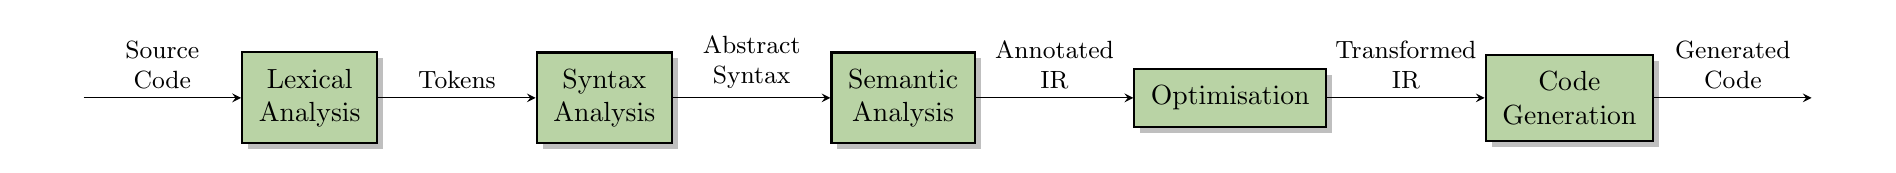
\begin{tikzpicture}[auto,
    ->,
  %  shorten >=2pt,
    >=stealth,
]
    \node[inv] (0) []             {};
    \node[bb]  (1) [right = of 0, xshift=1cm] {Lexical \\ Analysis};
    \node[bb]  (2) [right = of 1, xshift=1cm] {Syntax \\ Analysis};
    \node[bb]  (3) [right = of 2, xshift=1cm] {Semantic \\ Analysis};
    \node[bb]  (4) [right = of 3, xshift=1cm] {Optimisation};
    \node[bb]  (5) [right = of 4, xshift=1cm] {Code \\ Generation};
    \node[inv] (6) [right = of 5, xshift=1cm] {};
\begin{small}
    \path (0) edge node[align=center] {Source \\ Code}     (1)
          (1) edge node[align=center] {Tokens}             (2)
          (2) edge node[align=center] {Abstract \\ Syntax} (3)
          (3) edge node[align=center] {Annotated \\ IR}    (4)
          (4) edge node[align=center] {Transformed \\ IR}  (5)
          (5) edge node[align=center] {Generated \\ Code}  (6)
    ;

\end{small}
  \end{tikzpicture}
}

\end{center}

\end{frame}
% frame end %%%%%%%%%%%%%%%%%%%%%%%%

% frame begin %%%%%%%%%%%%%%%%%%%%%%%%
\begin{frame}{Lexical Analysis}
{Example -- Natural Languages}

\begin{center}
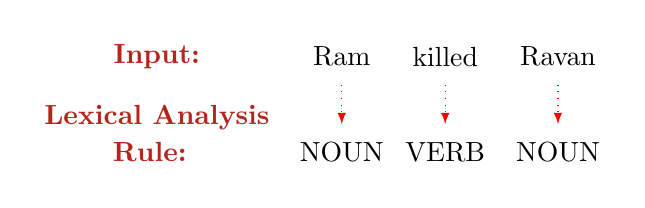
\begin{tikzpicture}
\node[inv](ram){Ram};
\node[inv, right=0.1cm of ram](killed){killed};
\node[inv, right=0.1cm of killed](ravan){Ravan};
\node[inv, left=of ram](inp){\textbf{\color{BrickRed}Input:}};
\pause
\node[inv, below=0.5cm of ram](n1){NOUN};
\node[inv, below=0.5cm of killed](v){VERB};
\node[inv, below=0.5cm of ravan](n2){NOUN};
\node[inv, left=of n1](rule){\textbf{\color{BrickRed}Rule:}};
\pause
\draw[-latex, Red, dotted] (ram) -- (n1);
\draw[-latex, Red, dotted] (killed) -- (v);
\draw[-latex, Red, dotted] (ravan) -- (n2);
\node[inv, below=0.1em of inp]{\textbf{\color{BrickRed}Lexical Analysis}};
\end{tikzpicture}
\end{center}
\end{frame}
% frame end %%%%%%%%%%%%%%%%%%%%%%%%

% frame begin %%%%%%%%%%%%%%%%%%%%%%%%
\begin{frame}{Lexical Analysis}
{Example -- Programming Languages}


\begin{center}
\resizebox{\textwidth}{!}{%
\begin{tikzpicture}[auto,
    ->,
  %  shorten >=2pt,
    >=stealth,
]
    \node[inv] (1)  [right = of 0]  {\texttt{int}};
    \node[inv] (2)  [right = of 1]  {\texttt{main}};
    \node[inv] (3)  [right = of 2]  {\texttt{(}};
    \node[inv] (4)  [right = of 3]  {\texttt{)}};
    \node[inv] (5)  [right = of 4]  {\texttt{\{}};
    \node[inv] (6)  [right = of 5]  {\texttt{printf}};
    \node[inv] (7)  [right = of 6]  {\texttt{(}};
    \node[inv] (8)  [right = of 7]  {\texttt{Hello World!}};
    \node[inv] (9)  [right = of 8]  {\texttt{)}};
    \node[inv] (10) [right = of 9]  {\texttt{;}};
    \node[inv] (11) [right = of 10] {\texttt{\}}};

\pause
    \node[bb] (t1)  [below = of 1]  {KW \\ \texttt{int}};
    \node[bb] (t2)  [below = of 2]  {ID \\ \texttt{main}};
    \node[bb] (t3)  [below = of 3]  {\texttt{(}};
    \node[bb] (t4)  [below = of 4]  {\texttt{)}};
    \node[bb] (t5)  [below = of 5]  {\texttt{\{}};
    \node[bb] (t6)  [below = of 6]  {ID \\ \texttt{printf}};
    \node[bb] (t7)  [below = of 7]  {\texttt{(}};
    \node[bb] (t8)  [below = of 8]  {SL \\\texttt{Hello World!}};
    \node[bb] (t9)  [below = of 9]  {\texttt{)}};
    \node[bb] (t10) [below = of 10]  {\texttt{;}};
    \node[bb] (t11) [below = of 11] {\texttt{\}}};

\draw[-latex, Red, dotted] (1) -- (t1);
\draw[-latex, Red, dotted] (2) -- (t2);
\draw[-latex, Red, dotted] (3) -- (t3);
\draw[-latex, Red, dotted] (4) -- (t4);
\draw[-latex, Red, dotted] (5) -- (t5);
\draw[-latex, Red, dotted] (6) -- (t6);
\draw[-latex, Red, dotted] (7) -- (t7);
\draw[-latex, Red, dotted] (8) -- (t8);
\draw[-latex, Red, dotted] (9) -- (t9);
\draw[-latex, Red, dotted] (10) -- (t10);
\draw[-latex, Red, dotted] (11) -- (t11);
  \end{tikzpicture}
}

\end{center}

\myminorheader{Terminology}
\begin{itemize} 
\item \textbf{\color{BrickRed}Token classes/Tokens.} e.g. KW, ID, (, \} etc. 
\item \textbf{\color{BrickRed}Lexemes.} e.g. \texttt{"int"}, \texttt{"main"}, \texttt{"("}, \texttt{"\}"} etc. 
\end{itemize}
\end{frame}
% frame end %%%%%%%%%%%%%%%%%%%%%%%%

% frame begin %%%%%%%%%%%%%%%%%%%%%%%%
\begin{frame}{Specification of Token Classes}
{Example}

\begin{center}
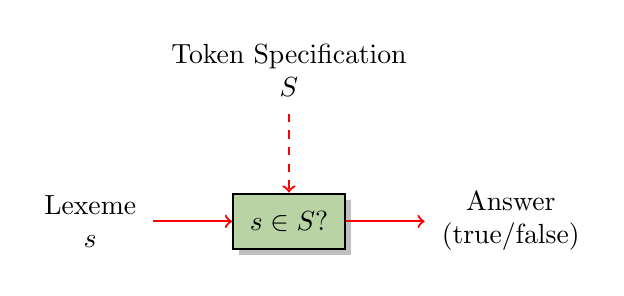
\begin{tikzpicture}
\node[inv](lexeme) {Lexeme \\ $s$};
\node[bb, right=of lexeme](la) {$s \in S?$};
\node[inv, above=of la](spec) {Token Specification \\ $S$};
\node[inv, right=of la](ans) {Answer \\ (true/false)};

\draw[->, Red, thick] (lexeme) -- (la);
\draw[->, Red, dashed, thick] (spec) -- (la);
\draw[->, Red, thick] (la) -- (ans);
\end{tikzpicture}
\end{center}

\pause
Specification ($S$) of token classes \pause -- \emph{regular expressions}
\end{frame}
% frame end %%%%%%%%%%%%%%%%%%%%%%%%

% frame begin %%%%%%%%%%%%%%%%%%%%%%%%
\begin{frame}[fragile]{Regular Expressions}
{Example -- identifier}
\begin{itemize}
	\item \textbf{\color{BrickRed}English:}
	\begin{itemize}
		\item Must comprise of only alphabetic character ($\alpha$)
	\end{itemize}
	\pause
	\item \textbf{\color{BrickRed}Regular Expression: }$\alpha+$
\end{itemize}
\end{frame}
% frame end %%%%%%%%%%%%%%%%%%%%%%%%


% frame begin %%%%%%%%%%%%%%%%%%%%%%%%
\begin{frame}[fragile]{Regular Expressions}
{Example -- identifier}
\begin{itemize}
	\item \textbf{\color{BrickRed}English:}
	\begin{itemize}
		\item Must start with an alphabetic character ($\alpha$)
		\item Subsequent letters can be alphabetic or numeric ($N$)
	\end{itemize}
	\pause
	\item \textbf{\color{BrickRed}Regular Expression: }$\alpha (\alpha | N)*$
\end{itemize}
\end{frame}
% frame end %%%%%%%%%%%%%%%%%%%%%%%%

% frame begin %%%%%%%%%%%%%%%%%%%%%%%%
\begin{frame}[fragile]{Regular Expressions}
{Rules of Construction}
\begin{enumerate}
	\item $\epsilon$ (empty symbol)
	\item Let $r$ and $s$ be two regular expressions:

\begin{scriptsize}
\begin{tabular}{c @{ \hspace{0.5cm} } c}
\begin{minipage}{0.4\textwidth}
		\begin{tabular}{l | l}
			\hline
			\textbf{\color{BrickRed}Expression} & \textbf{\color{BrickRed}Meaning} \\
			\hline
			$r | s$  & Choice        \\
			$rs$     & Concatenation \\
			$r\star$ & Zero or more  \\
			$r+$     & One or more   \\
			$r?$     & Zero or one   \\
		\end{tabular}		 
\end{minipage}	
&
\pause
\begin{minipage}{0.4\textwidth}
		\begin{tabular}{l | l}
			\hline
			\textbf{\color{BrickRed}Example} & \textbf{\color{BrickRed}Instance} \\
			\hline
			$\alpha | N$  & a, b, ..., 1, 2, ...        \\
			$rs$     & a1, b1, ..., a2, ... \\
			$\alpha\star$ & $\epsilon$, a, ab, aaa, ...  \\
			$N+$     & 1, 11, 12, ...   \\
			$N?$     & $\epsilon$, 1, 2, ...   \\
		\end{tabular}		 
\end{minipage}	
\end{tabular}
\end{scriptsize}
\end{enumerate}
\end{frame}
% frame end %%%%%%%%%%%%%%%%%%%%%%%%


% frame begin %%%%%%%%%%%%%%%%%%%%%%%%
\begin{frame}[fragile]{Regular Expressions}
{Example -- Identifier}
\begin{itemize}
	\item \textbf{English:}
	\begin{enumerate}
		\item Must start with an alphabetic character
		\item Subsequently, may have either an alphabetic character ($\alpha$), a numeric character ($N$), separated by zero or more underscores (\texttt{'\_'}).
	\end{enumerate}
	\pause
	\item \textbf{Regular Expression: }$\alpha\lbrace\lbrack(\alpha | N)$(\texttt{'\_'}$\star)\rbrack\star(\alpha | N)\rbrace?$
\end{itemize}
\end{frame}
% frame end %%%%%%%%%%%%%%%%%%%%%%%%

% frame begin %%%%%%%%%%%%%%%%%%%%%%%%
\begin{frame}[fragile]{Regular Expressions}
{Activity}
Regular expression for floating point numbers in C programming language

\end{frame}
% frame end %%%%%%%%%%%%%%%%%%%%%%%%

% frame begin %%%%%%%%%%%%%%%%%%%%%%%%
\begin{frame}{Implementation of Lexical Analysis}
{Finite State Automata}
\myminorheader{Example}

\textbf{NUMBER:}
\pause
\begin{center}
\resizebox{!}{0.2\textheight}{%
\begin{tikzpicture}[auto,
    ->,
    >=stealth
  ]
    \node[initial, state]   (0)                {$0$};
    \node[state, accepting]            (1) [right = of 0] {$1$};
%    \node[state, accepting] (2) [right = of 1] {$2^*$};
    
    \path (0) edge node {$digit$} (1)
%         (1) edge node {$other$} (2)
          (1) edge[loop above] node {$digit$} (1)
    ;
    \node (7) [right = of 2, xshift=-1cm] {return $NUMBER$};
    
    
  \end{tikzpicture}
}

\end{center}

\end{frame}
% frame end %%%%%%%%%%%%%%%%%%%%%%%%

% frame begin %%%%%%%%%%%%%%%%%%%%%%%%
\begin{frame}[fragile]{Regular Expressions}
{Regular Expressions and Finite State Automata}
\begin{itemize}
	\item Regular expressions are easy to use for specifying token classes but ... \pause hard to implement.
	\pause
	\item Finite state machines are easy to implement but ... \pause what about their correspondence with token classes?
	\pause
	\item Equivalent
	\item Let {R} be the set of all regular expressions, and let {F} be the set of all finite state automata.
	\[ \forall r \in {R}, \exists f \in {F} \text{ such that } {L}({r}) = {L}({f}) \]

	\[ \forall f \in {F}, \exists r \in {R}, \text{ such that } {L}({r}) = {L}({f}) \]	 
\end{itemize}

\pause
\begin{center}

\begin{tikzpicture}
\node[rectangle, draw=Red, fill=Red]{};
\end{tikzpicture}
\end{center}
\end{frame}
% frame end %%%%%%%%%%%%%%%%%%%%%%%%


% frame begin %%%%%%%%%%%%%%%%%%%%%%%%
\begin{frame}[fragile]{Lexical Analysis}
{Overview}
\begin{itemize}
	\item Finite state automata
	\item Implementation of finite state automata
	\item Implementation of lexical analysers: manual and automated generation
\end{itemize}
\end{frame}
% frame end %%%%%%%%%%%%%%%%%%%%%%%%

\end{document}
